%!TEX root = cscw2019-comic.tex
\section{Method}
\label{sec:Method}
In this study, we examine if the abstract comic can impact a decision with monetary consequence on Amazon Mechanical Turk. The persuasion task is to ask participants to make a charitable donation decision to the Organization for Autism Research with the real money. As we mentioned in earlier sections, four design principles guide us to choose the online charitable donation task. First, the online charitable donation is a kind of collective dilemma where study participants will receive no external/distant rewards based on their decision, which signifies the impact from the persuasive message in study participants' decision-making process. Second, encouraging people to donate is a single shot task that requires no habit formation, which protects us from several confounding variables such as life events and resource constraints (e.g., time). Third, with the advance in social network and internet, although the task is still challenging, charities or organizations nowadays solicit donations online textual messages (e.g., Wikipedia's fundraising banner), which makes our task ecologically valid. Fourth, online charitable donation requires no specialized knowledge. In our study, we choose the Organization for Autism Research as Autism Spectrum Disorder (ASD), is a well-known developmental disorder that impairs communication and behavior \cite{american2013diagnostic}. In other words, ASD provides basic interest for the participants to support the related charitable organization. In this section, we will introduce the experiment design and describe our study participants recruiting process.

%In this study, we examine if the abstract comic can impact a decision with monetary consequence. The aim of this study is to show the persuasiveness of the abstract comic in the real-life setting.  
%In contrast, the first study demonstrated that participants prefer messages in abstract comic form over text, but did not demonstrate persuasiveness.
% as more persuasive, it is unknown if the perceived persuasiveness can impact people's real-life decision making. So, we further studied the ability of abstract comics in persuading people to make decisions in real life. 
% In the second study, we conduct a field study on Amazon Mechanical Turk and compared the power between pure text messages and abstract comic messages in persuading people to donate with their real money. 
%In this section, we will introduce the experiment design and describe our study participants recruiting process.

\subsection{Experiment Design}
Since the main goal for this study is to compare the power of a persuasive message in two forms, the abstract comic and the text, we first constructed two experimental conditions, comic condition (see~\Cref{fig:basic three comic panel}) and text condition. In the comic condition, participants will read a message asking if they are willing to support a charity in a three-panel abstract comic strip, whereas in the text condition, participants will receive the same message in pure textual form. To test the idea of social proof, we then added a third condition, comic with the social proof, a three-panel comic that has the same content as the comic condition but added one line text that indicates the normative behavior (see~\Cref{fig:basic three comic social proof}).
% Additionally, we are also interested in if the abstract comic can leverage persuasive techniques to increase its persuasiveness. Hence, we incorporated the idea of social proof and created the third condition, social-proof-comic.

\begin{figure}[bt]
    \centering
    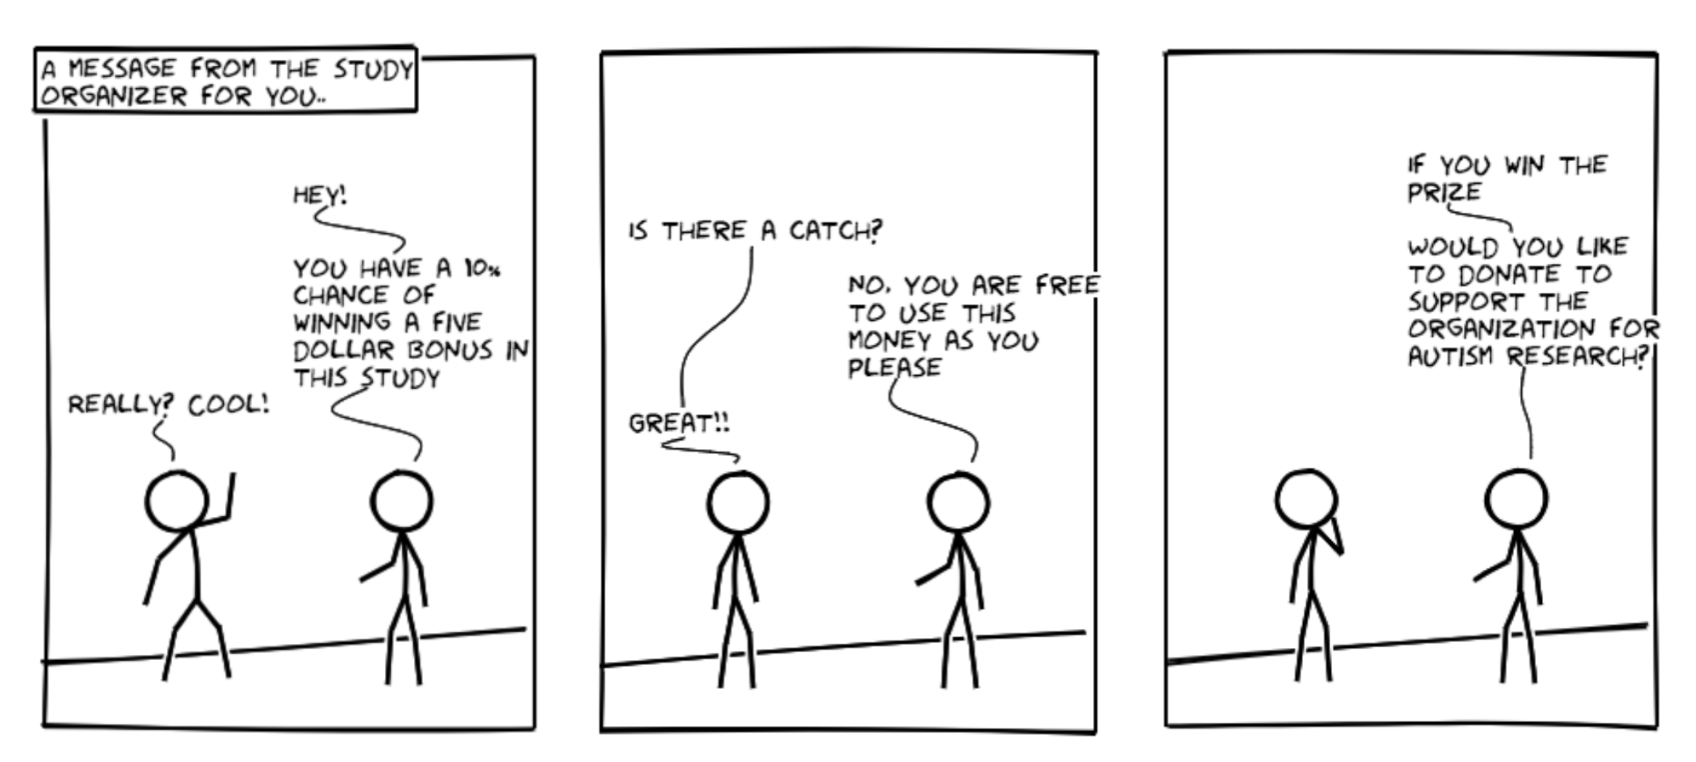
\includegraphics[width=\columnwidth]{./figures/abstract_comic.png}
    \caption{Messages in the abstract comic form. Same as the text messages, the three-panel comic strip communicates three major objectives, 1) Participants will have 10 \% of a chance winning \$ 5 bonus upon the completion of the study (see the first panel). 2) Participants are free to use the money as they please (see the second panel). and 3) Participants can donate this bonus to the Organization for Autism Research (OAR) (see the third panel).}
    \label{fig:basic three comic panel}
\end{figure}

The objectives of the persuasive message in all three conditions: persuading participants to donate to a charity from his/her own pocket. Similar to \textcite{lee2013does}, the money participants will use is part of their study compensation, a prospective bonus reward (10\% chance of winning \$5 bonus). We randomly assigned study participants to one of the three conditions; the participants are free to make a decision on the amount of donation, including not donating at all.

\subsection{Generating Comics}
In this study, we created a comic generator to generate the comic strips used in the study. The generator leveraged an open source comic library ~\cite{cmx.io} to generate comic figures and used ``rough.js'' \cite{rough.js} to generate other elements such as text bubble and outlines. The generator impersonates the style found on 'XKCD'~\cite{munroe2009xkcd} comic. Our focus is not the XKCD style, but the fact that the generated comic is abstract. We believe the generator has the potential to be further developed as a general framework to automatically synthesize pure-textual persuasive messages into abstract comic forms (we discuss this aspect further in section ~\Cref{sec:Discussion}).

\paragraph{Study Procedure} 
Once participants consented to join the study, we ask them if they are familiar with the Autism Spectrum Disorder (ASD). Then, each participant watched a short video produced by the Organization for Autism Research that promotes its fundraising activity "RUN FOR AUTISM". After watching the video, we asked participants to summarize the video using free text and ask them to provide their opinion about the effectiveness of the video. The recruiting message specifically mentioned this task of soliciting their opinion on video message's effectiveness. There are two main goals for this part of the study; First, we want to make sure prior familiarity with autism won't confound our study; Second, we want our main task less intrusive as soliciting charitable donation is not a common task on Amazon Mechanical Turk.  

We then randomly assigned participants to each of the three conditions and then ask them to read the corresponding persuasive message (text, three-panel comic, three-panel comic with social proof). In the message, we provided the participant with a 10\% chance of winning \$5 additional compensation. We also provide them with the opportunity to donate to the Organization for Autism Research (OAR) which is the charity mentioned in the video they watch as part of the study.

To best demonstrate the persuasiveness of the message itself, we diffused the responsibility of donation amount among all participants. Similar to ~\textcite{lee2013does}, before the participants make their decision, they read ``The total amount of money allocated to [the charity] by all the winning participants will be aggregated and donated at the end of the study.'' Then, we asked the participants to decide the amount of money they are willing to donate on a slider bar with \$0 and \$5 as two extreme ends. The default position of the slider bar is at the \$0 end.

Before leaving the study, we asked the participants to fill a demographic questionnaire about their gender, age, and education; the participants had the option of declining to state an answer for each question.

At the end of the study, we randomly chose 10\% of the participants, donated to OAR based on the participants' decision, and rewarded each chosen participant the part of the bonus that they wished to keep.

To gather the basic statistics to create social proof, we first ran a pilot study with the first two conditions ($n=60$) and used the donation statistics as part of the social proof message. In the pilot study, 87\% of the participants donated a non-zero amount. 



\begin{figure}[bt]
    \centering
    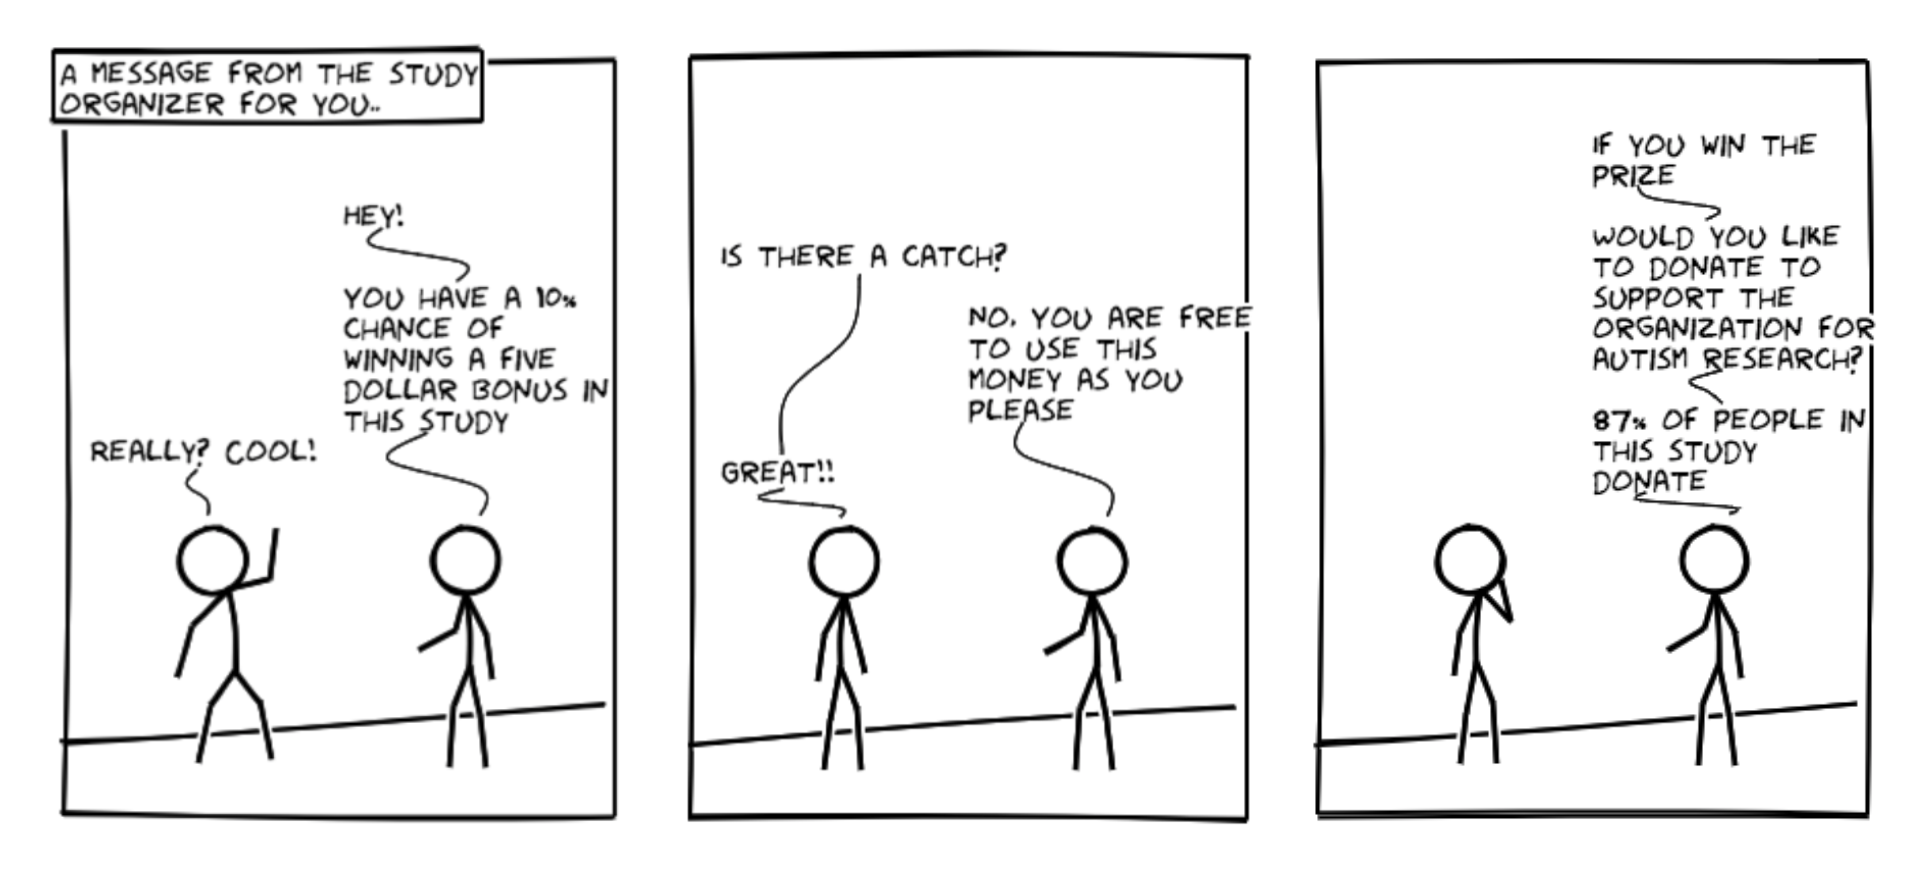
\includegraphics[width=\columnwidth]{./figures/social_proof.png}
    \caption{Messages with social proof. Additional to the three major objectives, the comic with social proof communicates the idea of the social proof at the third comic panel. The figure ``87\%'' comes from our pilot study}
    \label{fig:basic three comic social proof}
\end{figure}

\paragraph{Organization for Autism Research (OAR)}
To increase the realism of our study, the donation decision is not hypothetical and participants are rewarded based on their decision and we as study organizers donate to the Organization for Autism Research (OAR). We chose OAR as the charity in our study for three reasons. First, Autism Spectrum Disorder (ASD), is a well-known, serious developmental disorder that impairs communication and behavior. In other words, ASD provides basic interest for the participants to support the related charitable organization. Second, the Organization for Autism Research is one of the most visible ASD related organizations that helps individuals with autism and provides assistance to parents, families, teachers, and caregivers. The goal of OAR is clear and reputable so participants won't question the authenticity of our message's motive. Finally, we wished to avoid a charity associated with a life-threatening condition such as cancer as it may create an experimental confound: we don't know if someone donates because their intrinsic desire to help with a life-threatening situation. While ASD can have serious consequences on the well being of those who have it, the public perception is that ASD is not-life threatening. 

\paragraph{Persuasive Messages}
The persuasive messages communicate three major objectives, 1) Participants will have 10 \% of a chance winning \$ 5 bonus upon the completion of the study. 2) Participants are free to use the money as they please. and 3) Participants can donate this bonus to the Organization for Autism Research (OAR). Therefore, in the text condition, study participants will read the following message,
\begin{quote}
  \textit{You have a 10\% chance of winning a five dollar bonus in this study. You are free to use this money as you please. If you win the prize, would you like to donate to support the Organization for Autism Research?}
\end{quote}
In the two comic conditions, we created three-panel comic strips to communicate the \textit{same} text message. The three-panel comic strip allows us to leverage one of the most fascinating aspects of comics---storytelling~\cite{scott1993understanding}. 
%Since the first study did not show a convincing effect for framing, participant gesture, character distance and shading, we did not vary those conditions in this experiment. We set the inter-character distance to be medium, light background. 
Consistent with ``match on action'' technique~\cite{scott1993understanding}, we matched the panels on the gesture of the first character (the message recipient), while retaining a neutral gesture for the second character (who delivers the message). 

%We create the comic strip in a manner similar to the first study on preference.

% Each of the three panel communicates one major objective in the message. The comic strip is created in the similar fashion as in the first study on preference. As we learned from the first study that appropriate gestures will maximize the persuasiveness of the comics, we then chose the gesture that we believe best suit for the scenario see~\Cref{fig:basic three comic panel}.

In the comic with social proof condition, we created social-proof by adding one sentence on the last comic panel indicates the percentage of people in our study donated see~\Cref{fig:basic three comic social proof}. The percentage (87\%) corresponds to the number of people who donated a non-zero amount in the pilot study.

% \begin{figure*}
%  \subfloat[Messages in the abstract comic form]{%
%   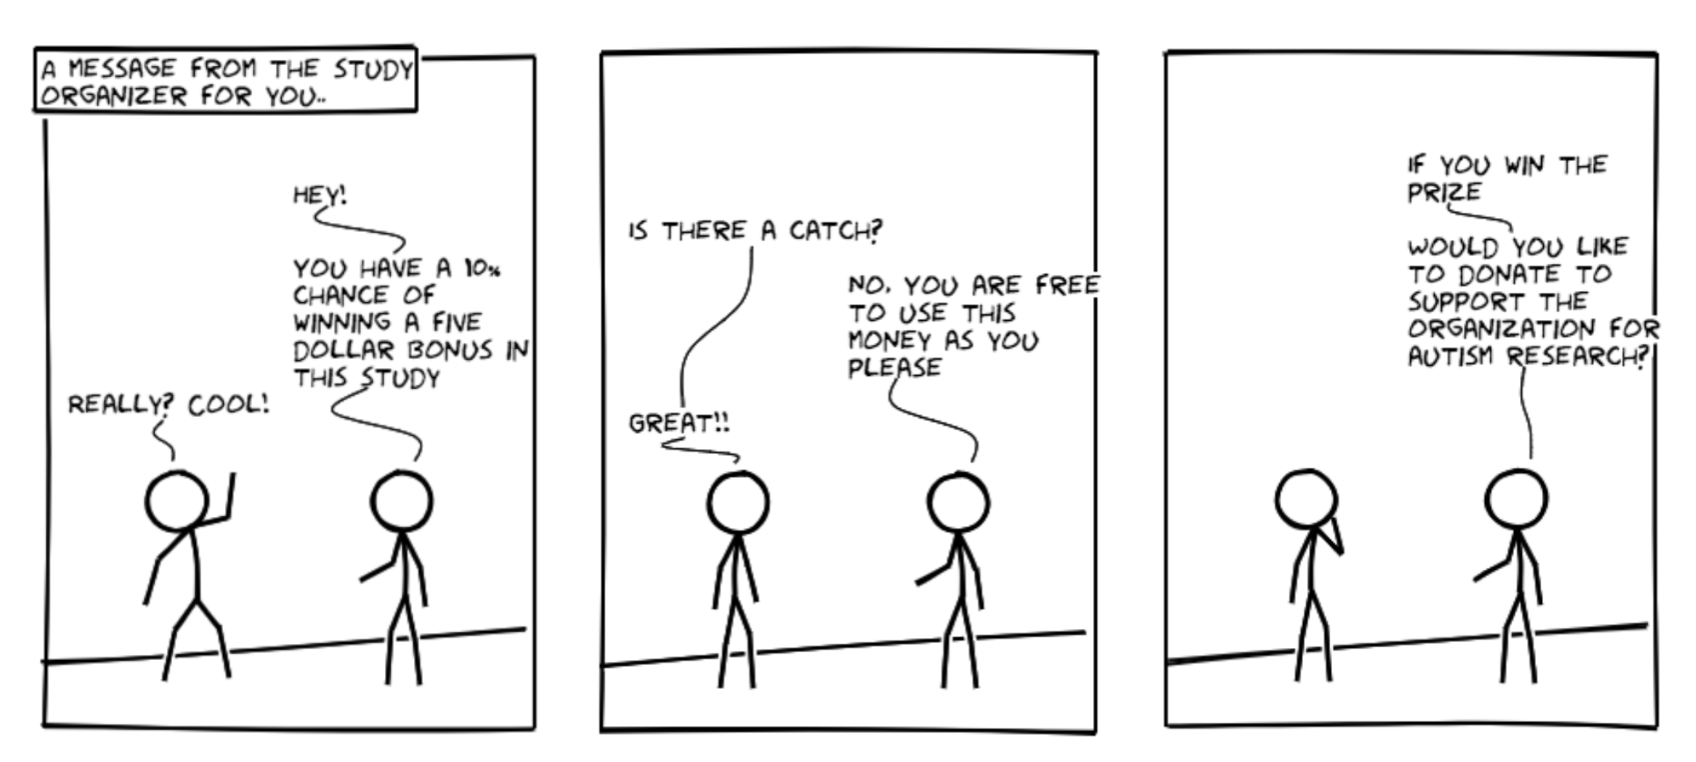
\includegraphics[width=0.5\textwidth]{./figures/abstract_comic.png}
%   } \hfill
%  \subfloat[Messages in the abstract comic form with social proof]{%
%   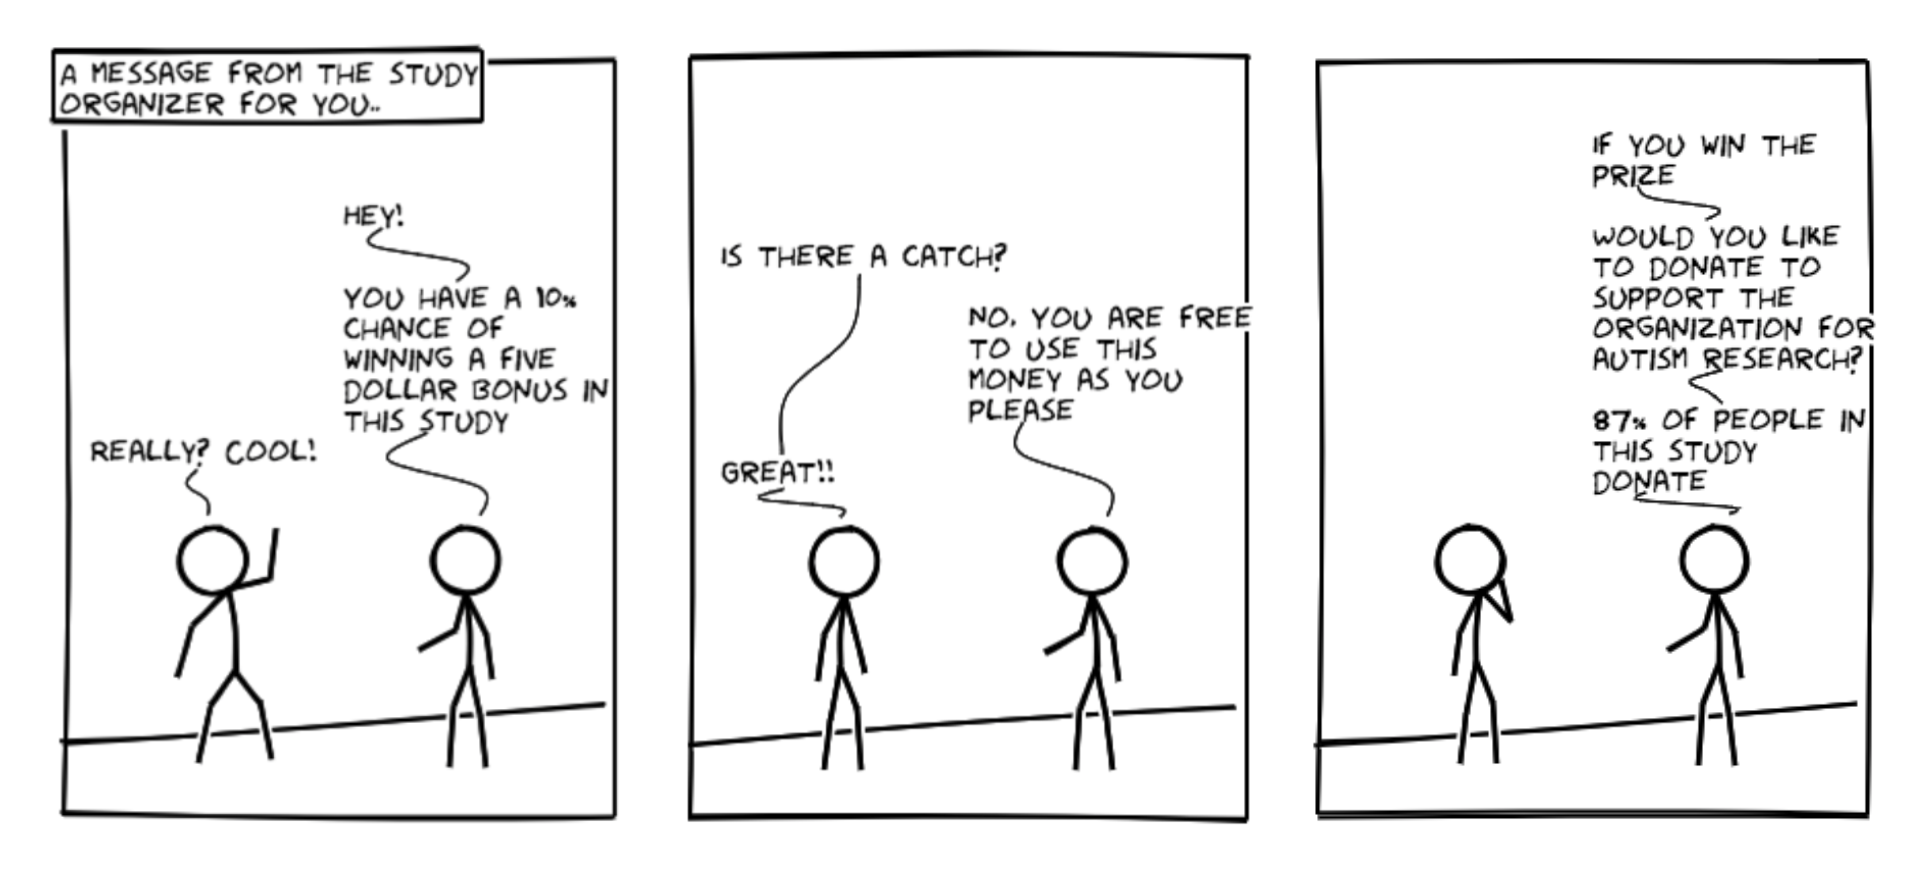
\includegraphics[width=0.5\textwidth]{./figures/social_proof.png}
%  }
%  \caption{The messages participants received in two abstract-comic conditions}
%  \label{fig:comic_messages_in_two_conditions}
% \end{figure*}

\subsubsection{Participants Recruitment}
In this study, we recruit our study participants from Amazon Mechanical Turk. Although Amazon Mechanical Turk is a crowdsourcing platform that has been widely used to gather human intelligence in AI research and social science experiments \cite{paolacci2010running, paolacci2014inside,berinsky2012evaluating}, we should be cautious when using such platform as the participant selection criteria is not transparent \cite{landers2015inconvenient}. In our study, we chose the Amazon Mechanical Turk for the following reasons. First, our persuasion task is about online charitable donation which targets internet users. Second, crowdsourcing platforms will help us reach a more diverse sample than using the researchers' own social network to attract participants \cite{mason2012conducting}. Third, the main motive for Amazon Mechanical Turk workers is monetary rewards \cite{berinsky2012evaluating}. In our study design, people will more sensitive to the monetary reward they may get and carefully make the donation decision, which makes our persuasive message more crucial. Fourth, to ensure transparency in participant's demographics, we have our own demographic questions. Thus, we believe it is valid for our experiment to use Amazon Mechanical Turk as our sample pool. 

We published our HITs on Amazon Mechanical Turk titled ``A short survey about communicating autism campaign ads``. The compensation was \$10/hr, and the workers would get these rewards regardless of their performance. To ensure quality, the HIT is limited to English Speakers and people who have a 95\% Approval Rate. On the HIT page, we instructed that repeated responses would be rejected. We told the participants that they would see a link to our experiment site. 
